\documentclass[twocolumn, 11pt]{article}%
\usepackage{amsmath, amssymb, esint, gensymb, hyperref, mathtools}
\usepackage{graphicx, cuted, geometry, float, scalerel, xcolor, xfrac}
\usepackage{enumitem}


\geometry{
    a4paper,
    total={170mm,260mm},
}

\begin{document}

\begin{strip}
  \vspace*{\dimexpr-\stripsep}
  \begin{center}
      \Large\textbf{FISIKA 2}\\
      \large{Pertemuan 1 - Minggu 10 (Presensi myITS kacau)}\\
      \large{\today}
   \end{center}
\end{strip}

\section{Gaya Gerak Listrik Induksi}
Inti dari pokok bahasan ini adalah menghasilkan \textbf{tegangan listrik}
dari medan magnet.

\subsection{Hukum Faraday}%
Hukum Faraday bermula dari 2 eksperimen

\subsubsection{Eksperimen Pertama}%
\begin{center}
    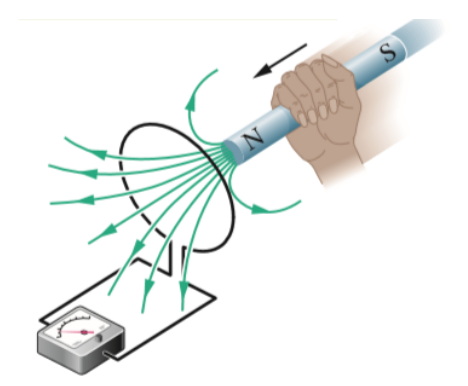
\includegraphics[width=130px]{1.png}\\
    \url{https://youtu.be/3HyORmBip-w}
\end{center}

Galvanometer (pengukur arus listrik kecil) mendeteksi arus listrik pada
loop kabel bila magnet digerakkan dengan cara tertentu di sekitar
kumparan.

\subsubsection{Eksperimen Kedua}%
\begin{center}
    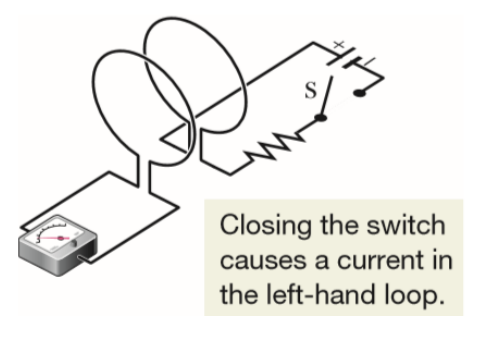
\includegraphics[width=130px]{2.png}
\end{center}

Galvanometer mendeteksi arus listrik pada loop sebelah kiri, pada saat
saklar S disambungkan (yang menyebabkan arus mengalir pada loop sebelah
kanan) atau pada saat saklar tersebut dibuka (memutus arus pada loop
kanan). Kumparan tidak digerakkan sama sekali.

\subsubsection{Perumusan}%
Faraday’s Law. Dengan notasi dari flux magnetik, kita bisa menjabarkan
Hukum Faraday dengan lebih kuantitatif, seperti berikut:

\begin{center}
    \textbf{
        Besar harga GGL (EMF) $\epsilon$ yang terinduksi pada loop
        konduktor sama dengan banyaknya perubahan flux magnetik $\Phi$ yang melewati loop tersebut dengan satuan waktu.
    }
\end{center}

\begin{align*}
    \epsilon &= -\frac{d\Phi}{dt}\\
    \epsilon &= -\frac{d(\vec B. \vec A)}{dt}\\
    \epsilon &= -\vec A.\ \frac{d(\vec B)}{dt}
\end{align*}

Tanda negatif (-) menunjukkan GGL yang timbul melawan penyebabnya (Gaya
Lorentz)

\begin{center}
    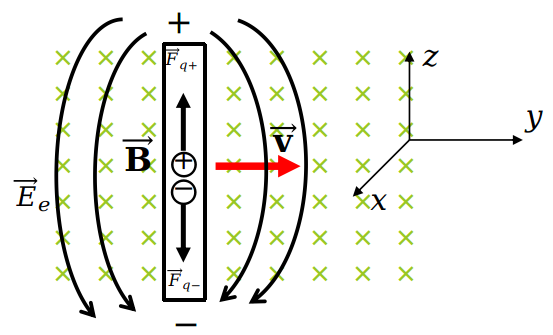
\includegraphics[width=200px]{3.png}
\end{center}
Pada kasus batang konduktor yang bergerak melintasi medan magnet yang
arahnya masuk bidang ($\times$) dan bergerak ke samping dengan kecepatan
$\vec v$. Maka
\[\vec F=q(\vec v \times \vec B) \]

Maka muatan positif pada batang logam tersebut akan bergerak ke atas
sesuai dengan rumus sebagai berikut:
\begin{align*}
    \overrightarrow{F_{q+}} &= qvB(\hat j \times -\hat i)\\
    \overrightarrow{F_{q+}} &= qvB(\hat k)
\end{align*}

Lalu muatan negatif pada batang logam tersebut akan bergerak ke bawah
sesuai dengan rumus sebagai berikut:
\begin{align*}
    \overrightarrow{F_{q-}} &= -qvB(\hat j \times -\hat i)\\
    \overrightarrow{F_{q-}} &= qvB(-\hat k)
\end{align*}

Sehingga ujung atas batang menjadi kutub positif (+), sedangkan ujung bawah
menjadi kutub negatif (-), yang menimbulkan medan elektrostatik
($\vec E_e$) yang arahnya melawan medan non elektrostatik ($\vec E_n$).\\

\begin{center}
    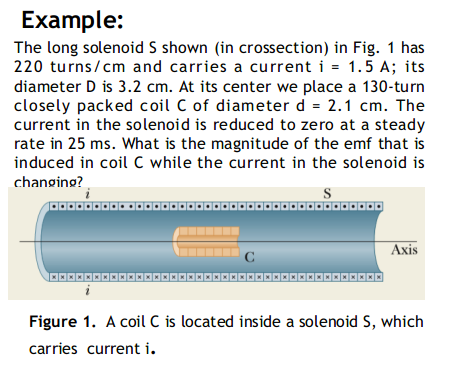
\includegraphics[width=200px]{4.png}\\
\end{center}

\textbf{JAWABAN:}

\begin{align*}
    \Phi &= B.A\\
    \Phi &= \frac{\mu_0iNA}{L}\\
\end{align*}

dengan
\[n=\frac{N}L =220\ \sfrac{\text{turns}}{\text{cm}} = 22000\
\sfrac{\text{turns}}{\text{m}} \]

\begin{center}
    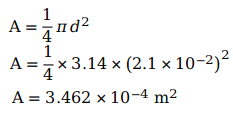
\includegraphics[width=150px]{5.png}
\end{center}

\begin{align*}
    \Phi &= \mu_0 inA\\
    \Phi &= 4\pi \times 10^{-7} \times 1.5 \times 22000 \times 3.462
    \times 10^{-4}\ \text{Wb}
\end{align*} 

\begin{center}
    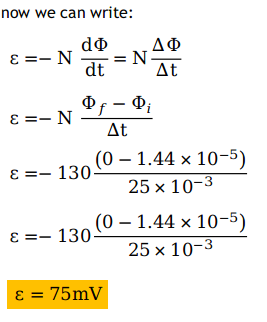
\includegraphics[width=150px]{6.png}
\end{center}

\subsubsection{GGL Induksi Pada Konduktor Bergerak}%

Batang konduktor AD dengan Panjang l bergerak ke kanan dengan kecepatan
$\vec v$, fluks awal yang dilingkupinya adalah:

\[ \Phi_1 = B.\text{ Luas ABCD} \]

Setelah bergerak selama $dt$ maka batang konduktor berpindah sejauh
$s=\vec v\ dt$, maka flux yang dilingkupinya menjadi:

\[ \Phi_2 = B.\text{ Luas A'BCD'} \]

Maka perubahan flux yang terjadi adalah:

\begin{align*}
    d\Phi &= \Phi_2 -\Phi_1\\
          &= B(\Delta \text{ Luas A'BCD'}-\Delta \text{ Luas ABCD})\\
          &= B(\Delta AA'DD')\\
          &= B(l.s)\\
          &= B(l.v.dt)\\
    \frac{d\Phi}{dt} &= -Blv
\end{align*}

Jadi, jika rumus di atas dimasukkan ke dalam hukum Faraday
\[\epsilon = -\frac{d\Phi}{dt} = Blv \]

\subsection{Dinamo Faraday}%
\begin{center}
    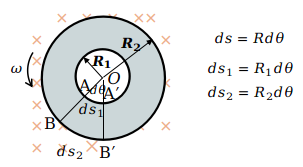
\includegraphics[width=200px]{8.png}
\end{center}

Misalkan besarnya simpangan sudut yang ditempuh cakram dalam selang waktu
$dt$, maka berkurangnya flux magnet:

\begin{align*}
    d\Phi &= -B(\text{ABB'A'})\\
    d\Phi &= -B(\Delta \text{OBB'} - \Delta \text{OAA'})\\
    d\Phi &= -B(\frac12R_2. ds_2 - \frac12 R_1. ds_1)\\
    d\Phi &= -B(\frac12R_2^2. d\theta - \frac12 R_1^2. d\theta)\\
    \frac{d\Phi}{dt} &= \frac{B}2 \frac{d\theta}{dt} (R_2^2-R_1^2)\\
    \frac{d\Phi}{dt} &= \frac{B}2 \omega (R_2^2-R_1^2)
\end{align*}

Dengan memasukkan persamaan terakhir ke dalam hukum Faraday, maka
\[ \epsilon=-\frac{d\Phi}{dt} = \frac{B}2 \omega (R_2^2-R_1^2) \]

\begin{center}
    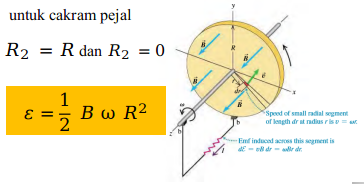
\includegraphics[width=200px]{9.png}
\end{center}

\subsection{Cara Menentukan Arah Arus Induksi}%
\begin{center}
    \url{https://youtu.be/1-aoGz5X_j0}
\end{center}

Sebuah batang magnet dipegang vertical di atas suatu loop horizontal ditunjukkan pada gambar. Kutub selatan magnet batang menghadap loop kawat, kemudian batang magnet dijatuhkan ke arah loop. Carilah arah arus yang lewat resistor,
\begin{enumerate}[label=\alph*).]
    \item Ketika batang magnet jatuh ke loop
    \item Setelah batang magnet melewati loop dan menjauhinya
\end{enumerate}

\begin{center}
    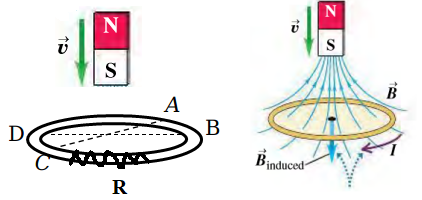
\includegraphics[width=200px]{10.png}
\end{center}

\textbf{PENYELESAIAN} 

\begin{enumerate}[label=\alph*).]
    \item Ketika batang magnet jatuh ke loop
\end{enumerate}

\begin{center}
    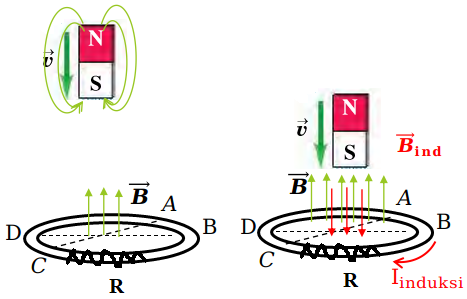
\includegraphics[width=200px]{11.png}
\end{center}

Saat awal (posisi magnet masih jauh), maka medan magnet yang menembus
cincin masih kecil dimisalkan 3 buah anak panah berwarna biru dengan arah
ke atas. Semakin mendekat, maka medan magnet semakin besar dimisalkan
menjadi 6 buah anak panah warna biru dengan arah ke atas.
Prinsipnya jumlah medan magnet awal dan akhir harus sama, sehingga agar
tetap sama dengan awal maka timbul 3 medan magnet induksi dengan arah ke
bawah (berwarna merah) yang dinamakan sebagai $B_{\text{induksi}}$
sehingga arah arus induksinya dari B ke C.\\


b). Setelah batang magnet melewati loop dan menjauhinya

\begin{center}
    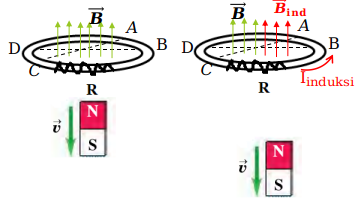
\includegraphics[width=200px]{12.png}
\end{center}

Saat awal (posisi magnet dekat), maka medan magnet yang menembus cincin
nilainya besar memisalkan 6 buah anak panah berwarna biru yang arahnya ke
atas. Semakin menjauh, maka medan magnet semakin kecil dimisalkan menjadi 3
buah anak panah warna biru dengan arah ke atas. Prinsipnya jumlah medan
magnet awal dan akhir harus sama, sehingga untuk mengimbanginya  timbul
medan magnet induksi dengan arah ke atas (3 anak panah berwarna merah) yang
dinamakan sebagai $B_{\text{induksi}}$ sehingga arah arus induksinya
dari C ke B.

\begin{center}
    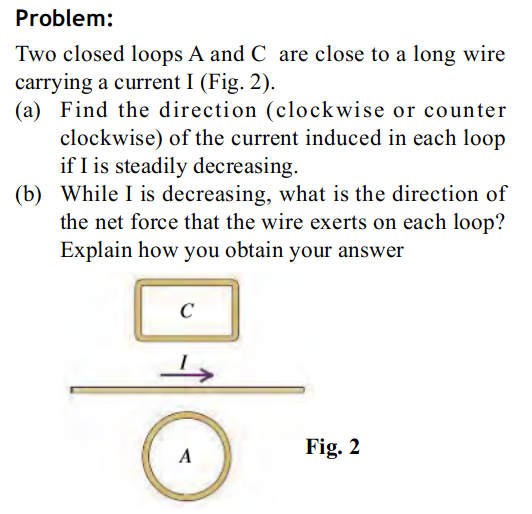
\includegraphics[width=240px]{13.png}
    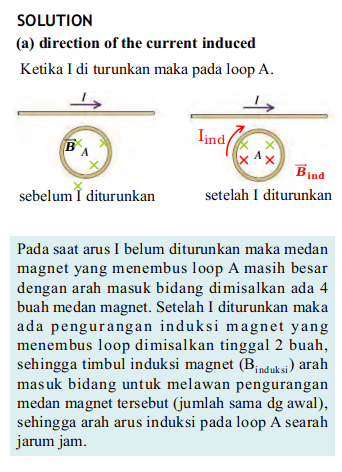
\includegraphics[width=240px]{14.png}
    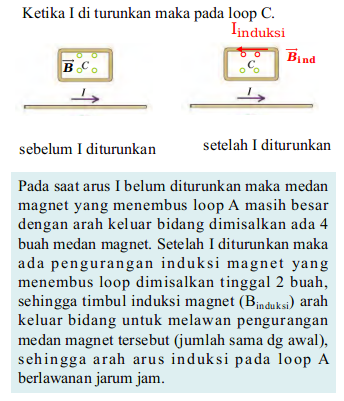
\includegraphics[width=240px]{15.png}
\end{center}

\subsection{Generator}%
\begin{center}
    \url{https://youtu.be/Ylgb8FFMgd4}
\end{center}

\subsubsection{Generator AC}%
\begin{center}
    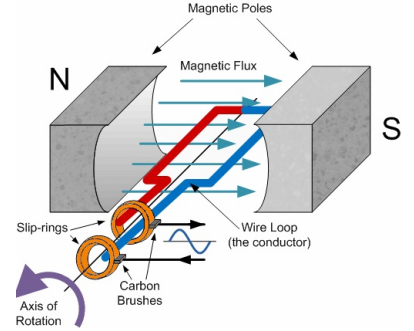
\includegraphics[width=180px]{16.png}
\end{center}

\subsubsection{Generator DC}%
\begin{center}
    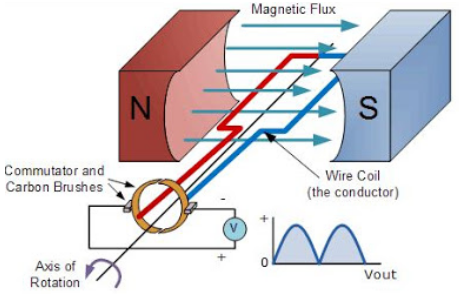
\includegraphics[width=180px]{17.png}
\end{center}

\subsubsection{Hukum Faraday Pada Generator}%
\begin{center}
    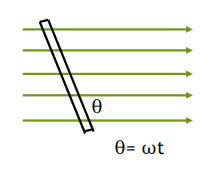
\includegraphics[width=100px]{18.png}
\end{center}

\begin{align*}
    \Phi &= \vec B.\vec A\\
    \Phi &= BA \cos \theta
\end{align*}

Maka
\begin{align*}
    \epsilon &= -N\frac{d\Phi}{dt}\\
    \epsilon &= -N\frac{d(\vec B.\vec A)}{dt}\\
    \epsilon &= -N\frac{d(BA \cos \theta)}{dt}\\
    \epsilon &= -NBA\frac{d(\cos \omega t)}{dt}\\
    \epsilon &= -NBA(-\sin \omega t)\omega\\
    \epsilon &= NBA\omega \sin \omega t\\
    \epsilon &= \epsilon_{max} \sin \omega t\\
\end{align*}

Jadi
\[\epsilon_{max} = NBA \omega \]
\end{document}
